\documentclass[11pt,addpoints,answers]{exam}

%-----------------------------------------------------------------------------
% PACKAGES AND OTHER DOCUMENT CONFIGURATIONS
%-----------------------------------------------------------------------------

\usepackage[margin=1in]{geometry}
\usepackage{amsmath, amsfonts}
\usepackage{enumerate}
\usepackage{graphicx}
\usepackage{titling}
\usepackage{url}
\usepackage{xfrac}
\usepackage{natbib}
\usepackage{amssymb}
\usepackage{amsthm}
\usepackage{paralist}
\usepackage{epstopdf}
\usepackage{tabularx}
\usepackage{longtable}
\usepackage{multirow}
\usepackage{multicol}
\usepackage[colorlinks=true,urlcolor=blue]{hyperref}
\usepackage{algorithm}
\usepackage{algorithmicx}
\usepackage[noend]{algpseudocode}
\usepackage{float}
\usepackage{enumerate}
\usepackage{array}
\usepackage{environ}
\usepackage{times}
\usepackage{textcomp}
\usepackage{caption}
\usepackage{parskip} % For NIPS style paragraphs.
\usepackage[compact]{titlesec} % Less whitespace around titles
\usepackage[inline]{enumitem} % For inline enumerate* and itemize*
\usepackage{datetime}
\usepackage{comment}
% \usepackage{minted}
\usepackage{lastpage}
\usepackage{color}
\usepackage{xcolor}
\usepackage[final]{listings}
\usepackage{tikz}
\usetikzlibrary{shapes,decorations}
\usepackage{framed}
\usepackage{booktabs}
\usepackage{cprotect}
\usepackage{verbatimbox}
\usepackage{multicol}
\usepackage{hyperref}
\usepackage{subcaption}
\usepackage{mathtools} % For drcases
\usepackage{cancel}
\usepackage[many]{tcolorbox}
\usepackage{soul}
\usepackage[bottom]{footmisc}
\usepackage{bm}
\usepackage{wasysym}

\usepackage{tikz}
\usetikzlibrary{arrows}
\usetikzlibrary{arrows.meta}
\usetikzlibrary{shapes.geometric}
\usetikzlibrary{positioning, arrows, automata, calc}

\newtcolorbox[]{your_solution}[1][]{
    % breakable,
    fit,
    enhanced,
    nobeforeafter,
    colback=white,
    title=Your Answer,
    sidebyside align=top,
    box align=top,
    #1
}

\lstset{frame=tb,
  language=Python,
  aboveskip=3mm,
  belowskip=3mm,
  showstringspaces=false,
  columns=flexible,
  basicstyle={\small\ttfamily},
  numbers=none,
  numberstyle=\tiny\color{gray},
  keywordstyle=\color{blue},
  commentstyle=\color{dkgreen},
  stringstyle=\color{mauve},
  breaklines=true,
  breakatwhitespace=true,
  tabsize=3
}


%%%%%%%%%%%%%%%%%%%%%%%%%%%%%%%%%%%%%%%%%%%
% Formatting for \CorrectChoice of "exam" %
%%%%%%%%%%%%%%%%%%%%%%%%%%%%%%%%%%%%%%%%%%%

\CorrectChoiceEmphasis{}
\checkedchar{\blackcircle}

%%%%%%%%%%%%%%%%%%%%%%%%%%%%%%%%%%%%%%%%%%%
% Rotated Column Headers                  %
%%%%%%%%%%%%%%%%%%%%%%%%%%%%%%%%%%%%%%%%%%%
\usepackage{adjustbox}
\usepackage{array}

%https://tex.stackexchange.com/questions/32683/rotated-column-titles-in-tabular

\newcolumntype{R}[2]{%
    >{\adjustbox{angle=#1,lap=\width-(#2)}\bgroup}%
    l%
    <{\egroup}%
}
\newcommand*\rot{\multicolumn{1}{R{45}{1em}}}% no optional argument here, please!

%%%%%%%%%%%%%%%%%%%%%%%%%%%%%%%%%%%%%%%%%%
% Custom commands                        %
%%%%%%%%%%%%%%%%%%%%%%%%%%%%%%%%%%%%%%%%%%

\newcommand{\vc}[1]{\boldsymbol{#1}}
\newcommand{\adj}[1]{\frac{d J}{d #1}}
\newcommand{\chain}[2]{\adj{#2} = \adj{#1}\frac{d #1}{d #2}}

\newcommand{\R}{\mathbb{R}}
\newcommand{\blackcircle}{\tikz\draw[black,fill=black] (0,0) circle (1ex);}
\renewcommand{\circle}{\tikz\draw[black] (0,0) circle (1ex);}

\newcommand{\emptysquare}{{\LARGE $\square$}\ \ }
\newcommand{\filledsquare}{{\LARGE $\blacksquare$}\ \ }
\newcommand{\emptycircle}{{\LARGE $\fullmoon$}\ \ }
\newcommand{\filledcircle}{{\LARGE $\newmoon$}\ \ }

\newcommand{\ntset}{test}

% mathcal
\newcommand{\Ac}{\mathcal{A}}
\newcommand{\Bc}{\mathcal{B}}
\newcommand{\Cc}{\mathcal{C}}
\newcommand{\Dc}{\mathcal{D}}
\newcommand{\Ec}{\mathcal{E}}
\newcommand{\Fc}{\mathcal{F}}
\newcommand{\Gc}{\mathcal{G}}
\newcommand{\Hc}{\mathcal{H}}
\newcommand{\Ic}{\mathcal{I}}
\newcommand{\Jc}{\mathcal{J}}
\newcommand{\Kc}{\mathcal{K}}
\newcommand{\Lc}{\mathcal{L}}
\newcommand{\Mc}{\mathcal{M}}
\newcommand{\Nc}{\mathcal{N}}
\newcommand{\Oc}{\mathcal{O}}
\newcommand{\Pc}{\mathcal{P}}
\newcommand{\Qc}{\mathcal{Q}}
\newcommand{\Rc}{\mathcal{R}}
\newcommand{\Sc}{\mathcal{S}}
\newcommand{\Tc}{\mathcal{T}}
\newcommand{\Uc}{\mathcal{U}}
\newcommand{\Vc}{\mathcal{V}}
\newcommand{\Wc}{\mathcal{W}}
\newcommand{\Xc}{\mathcal{X}}
\newcommand{\Yc}{\mathcal{Y}}
\newcommand{\Zc}{\mathcal{Z}}

% mathbb
\newcommand{\Ab}{\mathbb{A}}
\newcommand{\Bb}{\mathbb{B}}
\newcommand{\Cb}{\mathbb{C}}
\newcommand{\Db}{\mathbb{D}}
\newcommand{\Eb}{\mathbb{E}}
\newcommand{\Fb}{\mathbb{F}}
\newcommand{\Gb}{\mathbb{G}}
\newcommand{\Hb}{\mathbb{H}}
\newcommand{\Ib}{\mathbb{I}}
\newcommand{\Jb}{\mathbb{J}}
\newcommand{\Kb}{\mathbb{K}}
\newcommand{\Lb}{\mathbb{L}}
\newcommand{\Mb}{\mathbb{M}}
\newcommand{\Nb}{\mathbb{N}}
\newcommand{\Ob}{\mathbb{O}}
\newcommand{\Pb}{\mathbb{P}}
\newcommand{\Qb}{\mathbb{Q}}
\newcommand{\Rb}{\mathbb{R}}
\newcommand{\Sb}{\mathbb{S}}
\newcommand{\Tb}{\mathbb{T}}
\newcommand{\Ub}{\mathbb{U}}
\newcommand{\Vb}{\mathbb{V}}
\newcommand{\Wb}{\mathbb{W}}
\newcommand{\Xb}{\mathbb{X}}
\newcommand{\Yb}{\mathbb{Y}}
\newcommand{\Zb}{\mathbb{Z}}

% mathbf lowercase
\newcommand{\av}{\mathbf{a}}
\newcommand{\bv}{\mathbf{b}}
\newcommand{\cv}{\mathbf{c}}
\newcommand{\dv}{\mathbf{d}}
\newcommand{\ev}{\mathbf{e}}
\newcommand{\fv}{\mathbf{f}}
\newcommand{\gv}{\mathbf{g}}
\newcommand{\hv}{\mathbf{h}}
\newcommand{\iv}{\mathbf{i}}
\newcommand{\jv}{\mathbf{j}}
\newcommand{\kv}{\mathbf{k}}
\newcommand{\lv}{\mathbf{l}}
\newcommand{\mv}{\mathbf{m}}
\newcommand{\nv}{\mathbf{n}}
\newcommand{\ov}{\mathbf{o}}
\newcommand{\pv}{\mathbf{p}}
\newcommand{\qv}{\mathbf{q}}
\newcommand{\rv}{\mathbf{r}}
\newcommand{\sv}{\mathbf{s}}
\newcommand{\tv}{\mathbf{t}}
\newcommand{\uv}{\mathbf{u}}
\newcommand{\vv}{\mathbf{v}}
\newcommand{\wv}{\mathbf{w}}
\newcommand{\xv}{\mathbf{x}}
\newcommand{\yv}{\mathbf{y}}
\newcommand{\zv}{\mathbf{z}}

% mathbf uppercase
\newcommand{\Av}{\mathbf{A}}
\newcommand{\Bv}{\mathbf{B}}
\newcommand{\Cv}{\mathbf{C}}
\newcommand{\Dv}{\mathbf{D}}
\newcommand{\Ev}{\mathbf{E}}
\newcommand{\Fv}{\mathbf{F}}
\newcommand{\Gv}{\mathbf{G}}
\newcommand{\Hv}{\mathbf{H}}
\newcommand{\Iv}{\mathbf{I}}
\newcommand{\Jv}{\mathbf{J}}
\newcommand{\Kv}{\mathbf{K}}
\newcommand{\Lv}{\mathbf{L}}
\newcommand{\Mv}{\mathbf{M}}
\newcommand{\Nv}{\mathbf{N}}
\newcommand{\Ov}{\mathbf{O}}
\newcommand{\Pv}{\mathbf{P}}
\newcommand{\Qv}{\mathbf{Q}}
\newcommand{\Rv}{\mathbf{R}}
\newcommand{\Sv}{\mathbf{S}}
\newcommand{\Tv}{\mathbf{T}}
\newcommand{\Uv}{\mathbf{U}}
\newcommand{\Vv}{\mathbf{V}}
\newcommand{\Wv}{\mathbf{W}}
\newcommand{\Xv}{\mathbf{X}}
\newcommand{\Yv}{\mathbf{Y}}
\newcommand{\Zv}{\mathbf{Z}}

% bold greek lowercase
\newcommand{\alphav     }{\boldsymbol \alpha     }
\newcommand{\betav      }{\boldsymbol \beta      }
\newcommand{\gammav     }{\boldsymbol \gamma     }
\newcommand{\deltav     }{\boldsymbol \delta     }
\newcommand{\epsilonv   }{\boldsymbol \epsilon   }
\newcommand{\varepsilonv}{\boldsymbol \varepsilon}
\newcommand{\zetav      }{\boldsymbol \zeta      }
\newcommand{\etav       }{\boldsymbol \eta       }
\newcommand{\thetav     }{\boldsymbol \theta     }
\newcommand{\varthetav  }{\boldsymbol \vartheta  }
\newcommand{\iotav      }{\boldsymbol \iota      }
\newcommand{\kappav     }{\boldsymbol \kappa     }
\newcommand{\varkappav  }{\boldsymbol \varkappa  }
\newcommand{\lambdav    }{\boldsymbol \lambda    }
\newcommand{\muv        }{\boldsymbol \mu        }
\newcommand{\nuv        }{\boldsymbol \nu        }
\newcommand{\xiv        }{\boldsymbol \xi        }
\newcommand{\omicronv   }{\boldsymbol \omicron   }
\newcommand{\piv        }{\boldsymbol \pi        }
\newcommand{\varpiv     }{\boldsymbol \varpi     }
\newcommand{\rhov       }{\boldsymbol \rho       }
\newcommand{\varrhov    }{\boldsymbol \varrho    }
\newcommand{\sigmav     }{\boldsymbol \sigma     }
\newcommand{\varsigmav  }{\boldsymbol \varsigma  }
\newcommand{\tauv       }{\boldsymbol \tau       }
\newcommand{\upsilonv   }{\boldsymbol \upsilon   }
\newcommand{\phiv       }{\boldsymbol \phi       }
\newcommand{\varphiv    }{\boldsymbol \varphi    }
\newcommand{\chiv       }{\boldsymbol \chi       }
\newcommand{\psiv       }{\boldsymbol \psi       }
\newcommand{\omegav     }{\boldsymbol \omega     }

% bold greek uppercase
\newcommand{\Gammav     }{\boldsymbol \Gamma     }
\newcommand{\Deltav     }{\boldsymbol \Delta     }
\newcommand{\Thetav     }{\boldsymbol \Theta     }
\newcommand{\Lambdav    }{\boldsymbol \Lambda    }
\newcommand{\Xiv        }{\boldsymbol \Xi        }
\newcommand{\Piv        }{\boldsymbol \Pi        }
\newcommand{\Sigmav     }{\boldsymbol \Sigma     }
\newcommand{\Upsilonv   }{\boldsymbol \Upsilon   }
\newcommand{\Phiv       }{\boldsymbol \Phi       }
\newcommand{\Psiv       }{\boldsymbol \Psi       }
\newcommand{\Omegav     }{\boldsymbol \Omega     }

%%%%%%%%%%%%%%%%%%%%%%%%%%%%%%%%%%%%%%%%%%%
% Code highlighting with listings         %
%%%%%%%%%%%%%%%%%%%%%%%%%%%%%%%%%%%%%%%%%%%

\definecolor{bluekeywords}{rgb}{0.13,0.13,1}
\definecolor{greencomments}{rgb}{0,0.5,0}
\definecolor{redstrings}{rgb}{0.9,0,0}
\definecolor{light-gray}{gray}{0.95}

\newcommand{\MYhref}[3][blue]{\href{#2}{\color{#1}{#3}}}%

\definecolor{dkgreen}{rgb}{0,0.6,0}
\definecolor{gray}{rgb}{0.5,0.5,0.5}
\definecolor{mauve}{rgb}{0.58,0,0.82}

\lstdefinelanguage{Shell}{
  keywords={tar, cd, make},
  %keywordstyle=\color{bluekeywords}\bfseries,
  alsoletter={+},
  ndkeywords={python, py, javac, java, gcc, c, g++, cpp, .txt, octave, m, .tar},
  %ndkeywordstyle=\color{bluekeywords}\bfseries,
  identifierstyle=\color{black},
  sensitive=false,
  comment=[l]{//},
  morecomment=[s]{/*}{*/},
  commentstyle=\color{purple}\ttfamily,
  %stringstyle=\color{red}\ttfamily,
  morestring=[b]',
  morestring=[b]",
  backgroundcolor = \color{light-gray}
}

\lstset{columns=fixed, basicstyle=\ttfamily,
    backgroundcolor=\color{light-gray},xleftmargin=0.5cm,frame=tlbr,framesep=4pt,framerule=0pt}


%%%%%%%%%%%%%%%%%%%%%%%%%%%%%%%%%%%%%%%%%%%
% Custom box for highlights               %
%%%%%%%%%%%%%%%%%%%%%%%%%%%%%%%%%%%%%%%%%%%

% Define box and box title style
\tikzstyle{mybox} = [fill=blue!10, very thick,
    rectangle, rounded corners, inner sep=1em, inner ysep=1em]

% \newcommand{\notebox}[1]{
% \begin{tikzpicture}
% \node [mybox] (box){%
%     \begin{minipage}{\textwidth}
%     #1
%     \end{minipage}
% };
% \end{tikzpicture}%
% }

\NewEnviron{notebox}{

\begin{tikzpicture}
\node [mybox] (box){
    \begin{minipage}{\textwidth}
        \BODY
    \end{minipage}
};
\end{tikzpicture}
}

%%%%%%%%%%%%%%%%%%%%%%%%%%%%%%%%%%%%%%%%%%%
% Commands showing / hiding solutions     %
%%%%%%%%%%%%%%%%%%%%%%%%%%%%%%%%%%%%%%%%%%%

%% To HIDE SOLUTIONS (to post at the website for students), set this value to 0: 
\def\issoln{0}
% Some commands to allow solutions to be embedded in the assignment file.
\ifcsname issoln\endcsname \else \def\issoln{1} \fi
% Default to an empty solutions environ.
\NewEnviron{soln}{}{}
\if\issoln 1
% Otherwise, include solutions as below.
\RenewEnviron{soln}{
    \leavevmode\color{red}\ignorespaces
    % \textbf{Solution} \BODY
    \BODY
}{}
\fi

%% qauthor environment:
% Default to an empty qauthor environ.
\NewEnviron{qauthor}{}{}
%% To HIDE TAGS set this value to 0:
\def\showtags{0}
%%%%%%%%%%%%%%%%
\ifcsname showtags\endcsname \else \def\showtags{1} \fi
% Default to an empty tags environ.
\NewEnviron{tags}{}{}
\if\showtags 1
% Otherwise, include solutions as below.
\RenewEnviron{tags}{
    \fbox{
    \leavevmode\color{blue}\ignorespaces
    \textbf{TAGS:} \texttt{\url{\BODY}}
    }
    \vspace{-.5em}
}{}
\fi

%%%%%%%%%%%%%%%%%%%%%%%%%%%%%%%%%%%%%%%%%%%
% Commands for customizing the assignment %
%%%%%%%%%%%%%%%%%%%%%%%%%%%%%%%%%%%%%%%%%%%

\newcommand{\courseName}{10-301/10-601 Introduction to Machine Learning (Fall 2024)}
\newcommand{\hwName}{Homework 1: Background}
\newcommand{\dueDate}{Wednesday, September 4th}
\newcommand{\homeworktype}{\string hw1}

\title{\textsc{\hwName}
%\thanks{Compiled on \today{} at \currenttime{}}
} % Title


\author{\courseName\\
\url{http://www.cs.cmu.edu/~mgormley/courses/10601/} \\
OUT: Monday, August 26th \\
DUE: \dueDate{} \\ 
}

\date{}


%%%%%%%%%%%%%%%%%%%%%%%%%%%%%%%%%%%%%%%%%%%%%%%%%
% Useful commands for typesetting the questions %
%%%%%%%%%%%%%%%%%%%%%%%%%%%%%%%%%%%%%%%%%%%%%%%%%

\newcommand \expect {\mathbb{E}}
\newcommand \mle [1]{{\hat #1}^{\rm MLE}}
\newcommand \map [1]{{\hat #1}^{\rm MAP}}
\newcommand \argmax {\operatorname*{argmax}}
\newcommand \argmin {\operatorname*{argmin}}
\newcommand \code [1]{{\tt #1}}
\newcommand \datacount [1]{\#\{#1\}}
\newcommand \ind [1]{\mathbb{I}\{#1\}}

%%%%%%%%%%%%%%%%%%%%%%%%%%
% Document configuration %
%%%%%%%%%%%%%%%%%%%%%%%%%%

% Don't display a date in the title and remove the white space
\predate{}
\postdate{}
\date{}

% Don't display an author and remove the white space
%\preauthor{}
%\postauthor{}

% Solo and group questions
\newcommand{\solo}{\textbf{[SOLO]} }
\newcommand{\group}{\textbf{[GROUP]} }

% Question type commands
\newcommand{\sall}{\textbf{Select all that apply: }}
\newcommand{\sone}{\textbf{Select one: }}
\newcommand{\tf}{\textbf{True or False: }}

% AdaBoost commands
\newcommand{\trainerr}[1]{\hat{\epsilon}_S \left(#1\right)}
\newcommand{\generr}[1]{\epsilon \left(#1\right)}
\newcommand{\D}{\mathcal{D}}
\newcommand{\margin}{\text{margin}}
\newcommand{\sign}{\text{sign}}
\newcommand{\PrS}{\hat{\Pr_{(x_i, y_i) \sim S}}}
\newcommand{\PrSinline}{\hat{\Pr}_{(x_i, y_i) \sim S}}  % inline PrS

% Abhi messing around with examdoc
\qformat{\textbf{{\Large \thequestion \; \; \thequestiontitle \ (\totalpoints \ points)}} \hfill}
\renewcommand{\thequestion}{\arabic{question}}
\renewcommand{\questionlabel}{\thequestion.}

\renewcommand{\thepartno}{\arabic{partno}}
\renewcommand{\partlabel}{\thepartno.}
\renewcommand{\partshook}{\setlength{\leftmargin}{0pt}}

\renewcommand{\thesubpart}{\alph{subpart}}
\renewcommand{\subpartlabel}{(\thesubpart)}

\renewcommand{\thesubsubpart}{\roman{subsubpart}}
\renewcommand{\subsubpartlabel}{\thesubsubpart.}

% copied from stack overflow, as all good things are
\newcommand\invisiblesection[1]{%
  \refstepcounter{section}%
  \addcontentsline{toc}{section}{\protect\numberline{\thesection}#1}%
  \sectionmark{#1}}

% quite possibly the worst workaround i have made for this class
\newcommand{\sectionquestion}[1]{
\titledquestion{#1}
\invisiblesection{#1}
~\vspace{-1em}
}

%%%%%%%%%%%%%%%%%%%%%%%%%%%%%%%%%%%%%%%%%%%
% New Environment for Pseudocode          %
%%%%%%%%%%%%%%%%%%%%%%%%%%%%%%%%%%%%%%%%%%%

% Python style for highlighting
\DeclareFixedFont{\ttb}{T1}{txtt}{bx}{n}{10} % for bold
\DeclareFixedFont{\ttm}{T1}{txtt}{m}{n}{10}  % for normal

\definecolor{deepblue}{rgb}{0,0,0.5}
\definecolor{deepred}{rgb}{0.6,0,0}
\definecolor{deepgreen}{rgb}{0,0.5,0}

\newcommand\pythonstyle{\lstset{
language=Python,
basicstyle=\ttm,
morekeywords={self},              % Add keywords here
keywordstyle=\ttb\color{deepblue},
emphstyle=\ttb\color{deepred},    % Custom highlighting style
stringstyle=\color{deepgreen},
frame=tb,                         % Any extra options here
showstringspaces=false,
xleftmargin=0pt
}}

% Python environment
\lstnewenvironment{your_code_solution}[1][]
{
\pythonstyle
\lstset{#1}
}
{}

\newtcolorbox[]{your_code_solution_outer}[1][]{
    % breakable,
    enhanced,
    nobeforeafter,
    colback=white,
    title=Your Answer,
    sidebyside align=top,
    box align=top,
    #1
}

% Note from Matt: This should allow us to get down to just 
% one your_code_solution, but isn't working properly yet.
%
% \usepackage{keycommand}
% \newkeyenvironment{your_code_solution}[height=2cm,width=10cm,title={}][0]
% {
%     \begin{your_code_solution_outer}[height=\commandkey{height}, width=\commandkey{width}, title={\commandkey{title}}]
%     % Put your solution in the your_code_solution environment
%     \begin{your_code_solution_inner}
% }
% {
%     \end{your_code_solution_inner}
%     \end{your_code_solution_outer}
% }

%%%%%%%%%%%%%%%%%%
% Begin Document %
%%%%%%%%%%%%%%%%%% 

%%%%%%%%%%%%%%%%%%
% Begin Document %
%%%%%%%%%%%%%%%%%% 

\begin{document}

\maketitle

\section*{START HERE: Instructions}
\begin{itemize}
\item \textbf{Collaboration policy:} Collaboration on solving the homework is allowed, after you have thought about the problems on your own. It is also OK to get clarification (but not solutions) from books or online resources, again after you have thought about the problems on your own. There are two requirements: first, cite your collaborators fully and completely (e.g., ``Jane explained to me what is asked in Question 2.1''). Second, write your solution {\em independently}: close the book and all of your notes, and send collaborators out of the room, so that the solution comes from you only.  See the Academic Integrity Section on the course site for more information: \url{http://www.cs.cmu.edu/~mgormley/courses/10601/syllabus.html#7-academic-integrity-policies}

\item\textbf{Late Submission Policy:} See the late submission policy here: \url{http://www.cs.cmu.edu/~mgormley/courses/10601/syllabus.html#late-homework-policy}

\item\textbf{Submitting your work:} 

\begin{itemize}

% Since we are not using Canvas this semester.
% \item \textbf{Canvas:} We will use an online system called Canvas for short answer and multiple choice questions. You can log in with your Andrew ID and password. (As a reminder, never enter your Andrew password into any website unless you have first checked that the URL starts with "https://" and the domain name ends in ".cmu.edu" -- but in this case it's OK since both conditions are met).  You may only \textbf{submit once} on canvas, so be sure of your answers before you submit.  However, canvas allows you to work on your answers and then close out of the page and it will save your progress.  You will not be granted additional submissions, so please be confident of your solutions when you are submitting your assignment.

\item \textbf{Programming:} You will submit your code for programming questions on the homework to Gradescope (\url{https://gradescope.com}). After uploading your code, our grading scripts will autograde your assignment by running your program on a virtual machine (VM). When you are developing, check that the version number of the programming language environment (e.g. Python 3.9.12) and versions of permitted libraries (e.g.  \texttt{numpy} 1.23.0) match those used on Gradescope. You have a \textbf{total of 10 Gradescope programming submissions.} Use them wisely. In order to not waste code submissions, we recommend debugging your implementation on your local machine (or the linux servers) and making sure your code is running correctly first before any Gradescope coding submission. {\color{red} The above is true for future assignments, but this one allows \textbf{unlimited submissions.}}

\item \textbf{Written:} For written problems such as short answer, multiple choice, derivations, proofs, or plots, we will be using Gradescope (\url{https://gradescope.com/}). Please use the provided template. Submissions can be handwritten onto the template, but should be labeled and clearly legible. If your writing is not legible, you will not be awarded marks. Alternatively, submissions can be written in LaTeX. Regrade requests can be made, however this gives the TA the opportunity to regrade your entire paper, meaning if additional mistakes are found then points will be deducted.
Each derivation/proof should be  completed on a separate page. For short answer questions you \textbf{should not} include your work in your solution.  If you include your work in your solutions, your assignment may not be graded correctly by our AI assisted grader. {\color{red} For this assignment only, if you answer at least 90\% of the written questions correctly, you get full marks on the written portion of this assignment. For this assignment only, \textbf{we will offer two rounds of grading}. The first round of grading will happen immediately following the due date specified above. We will then release your grades to you and if you got less than 90\% on the written questions, you will be allowed to submit once again by a second due date. The exact due date for the second round will be announced after we release the first round grades. }

\end{itemize}

\item \textbf{Materials:} The data that you will need in order to complete this assignment is posted along with the writeup and template on the course website.

\end{itemize}

%Homework 9 will be on Gradescope, but will be "Canvas-style"- all problems will be multiple choice, select all that apply, or numerical answer. 

For multiple choice or select all that apply questions, shade in the box or circle in the template document corresponding to the correct answer(s) for each of the questions. For \LaTeX{} users, replace \lstinline{\choice} with \lstinline{\CorrectChoice} to obtain a shaded box/circle, and don't change anything else.\clearpage

\section*{Instructions for Specific Problem Types}

For ``Select One" questions, please fill in the appropriate bubble completely:

\begin{quote}
\textbf{Select One:} Who taught this course?
    \begin{checkboxes}
     \CorrectChoice Matt Gormley
     \choice Marie Curie
     \choice Noam Chomsky
    \end{checkboxes}
\end{quote}

If you need to change your answer, you may cross out the previous answer and bubble in the new answer:

\begin{quote}
\textbf{Select One:} Who taught this course?
    {
    \begin{checkboxes}
     \CorrectChoice Henry Chai 
     \choice Marie Curie \checkboxchar{\xcancel{\blackcircle}{}}
     \choice Noam Chomsky 
    \end{checkboxes}
    }
\end{quote}

For ``Select all that apply" questions, please fill in all appropriate squares completely:

\begin{quote}
\textbf{Select all that apply:} Which are instructors for this course?
    {%
    \checkboxchar{$\Box$} \checkedchar{$\blacksquare$} % change checkbox style locally
    \begin{checkboxes}
    \CorrectChoice Matt Gormley  
    \CorrectChoice Henry Chai
    \choice Isaac Newton
    \choice I don't know
    \end{checkboxes}
    }
\end{quote}

Again, if you need to change your answer, you may cross out the previous answer(s) and bubble in the new answer(s):

\begin{quote}
\textbf{Select all that apply:} Which are the instructors for this course?
    {%
    \checkboxchar{\xcancel{$\blacksquare$}} \checkedchar{$\blacksquare$} % change checkbox style locally
    \begin{checkboxes}
    \CorrectChoice Matt Gormley 
    \CorrectChoice Henry Chai
    \choice Isaac Newton
    \choice I don't know
    \end{checkboxes}
    }
\end{quote}

For questions where you must fill in a blank, please make sure your final answer is fully included in the given space. You may cross out answers or parts of answers, but the final answer must still be within the given space.

\begin{quote}
\textbf{Fill in the blank:} What is the course number?

\begin{tcolorbox}[fit,height=1cm, width=4cm, blank, borderline={1pt}{-2pt},nobeforeafter]
    \begin{center}\huge10-601\end{center}
    \end{tcolorbox}\hspace{2cm}
    \begin{tcolorbox}[fit,height=1cm, width=4cm, blank, borderline={1pt}{-2pt},nobeforeafter]
    \begin{center}\huge10-\xcancel{6}301\end{center}
    \end{tcolorbox}
\end{quote}
\clearpage

\section{Programming: Majority Vote Classifier [30 Points]} 

\subsection{Introduction}
The goal of this assignment is to ensure that you:
\begin{enumerate}
    \item Have a way to edit and test your code (i.e. a text editor and compiler/interpreter)
    \item Are familiar with submitting to Gradescope
    \item Are familiar with file I/O and standard output in Python
\end{enumerate}

\textbf{Warning:} This handout assumes that you are using a Unix command prompt (with \texttt{zsh, bash, csh} or similar). Windows commands may differ slightly.

\subsection{Majority Vote Classifier}

\subsubsection{Algorithm}


This assignment requires you to implement a Majority Vote Classifier.  Your algorithm should calculate the most common label in the data, ``predict'' that label for each given point in the dataset, and calculate the error rate for the classifier's predictions. You may assume that the output class label is always binary. 

The training procedure should store the label used for prediction at test time. In the case of a tie, output the value that is numerically higher (or comes \emph{last} alphabetically- ie. in a tie between Apples and Bananas, you would return Bananas). At test time, each example should be passed through the classifier. Its predicted label becomes the label most commonly occurring in the train set. 

\emph{Looking ahead:} This simple algorithm acts as a small component of the Decision \emph{Tree} that you will implement in the next homework assignment. We hope that you will employ best practices when coding so that you can re-use your own code here in the next assignment. A Majority Vote Classifier is simply a decision tree of depth zero (it predicts a class label for the input instance based on the most commonly occurring label present in the data).

\subsubsection{The Datasets}
\label{sec:data}

\paragraph{Materials} Download the zip file from course website, which contains all the data that you will need in order to complete this assignment.

\paragraph{Datasets}

The handout contains two datasets. Each one contains attributes and labels and is already split into training and testing data. The first row of each \lstinline{.tsv} file contains the name of each attribute, and \emph{the class label is always the last column}.

\begin{enumerate}
\item \textbf{heart:}
    The first task is to predict whether a patient has been (or will be) diagnosed with heart disease, based on available patient information. The attributes (aka. features) are: 
    \begin{enumerate}
        \item \lstinline{sex}: The sex of the patient---1 if the patient is male, and 0 if the patient is female.
        \item \lstinline{chest_pain}: 1 if the patient has chest pain, and 0 otherwise.
        \item \lstinline{high_blood_sugar}: 1 if the patient has high blood sugar ($>$120 mg/dl fasting), or 0 otherwise.
        \item \lstinline{abnormal_ecg}: 1 if exercise induced angina in the patient, and 0 otherwise. Angina is a type of severe chest pain.
        \item \lstinline{flat_ST}: 1 if the patient's ST segment (a section of an ECG) was flat during exercise, or 0 if it had some slope.
        \item \lstinline{fluoroscopy}: 1 if a physician used fluoroscopy, and 0 otherwise. Fluoroscopy is an imaging technique used to see the flow of blood through the heart.
        \item \lstinline{thalassemia}: 1 if the patient is known to have thalassemia, and 0 otherwise. Thalassemia is a blood disorder that may impair the oxygen-carrying capacity of the patient's red blood cells.
        \item \lstinline{heart_disease}: 1 if the patient was diagnosed with heart disease, and 0 otherwise. This is the class label you should predict.
    \end{enumerate}
    The training data is in \lstinline{heart_train.tsv}, and the test data in \lstinline{heart_test.tsv}.
\item \textbf{education:}
    The second task is to predict the final grade for high school students. The attributes are student grades on 5 multiple choice assignments \emph{M1} through \emph{M5}, 4 programming assignments \emph{P1} through \emph{P4}, and the final exam \emph{F}. Values of 1 indicate that a student received an A, and 0 indicates that the student did not receive an A. The training data is in \newline \lstinline{education_train.tsv}, and the test data in \lstinline{education_test.tsv}.

\end{enumerate}

The handout zip file also contains the predictions and metrics from a reference implementation of a Majority Vote Classifier for the \textbf{heart} and \textbf{education} datasets (see subfolder \emph{example\_output}). You can check your own output against these to see if your implementation is correct.\footnote{Yes, you read that correctly: we are giving you the correct answers.}

\begin{notebox} \textbf{Note:}
For simplicity, all attributes are discretized into just two categories. This applies to all the datasets in the handout, as well as the additional datasets on which we will evaluate your Majority Vote Classifier.
\end{notebox}

\subsubsection{Command Line Arguments}

The autograder runs and evaluates the output from the files  generated, using the following command:

\begin{tabular}{ll}
\begin{lstlisting}[language=Shell]
$ python majority_vote.py [args...]

\end{lstlisting}
\end{tabular}

Where above \lstinline{[args...]} is a placeholder for five command-line arguments: 
\texttt{<train input> <test input> <train out> <test out> <metrics out>}. These arguments are described in detail below:
\begin{enumerate}
\item \lstinline{<train input>}: path to the training input \lstinline{.tsv} file 
\item \lstinline{<test input>}: path to the test input \lstinline{.tsv} file 
\item \lstinline{<train out>}: path of output \lstinline{.txt} file to which the predictions on the \textit{training} data should be written 
\item \lstinline{<test out>}: path of output \lstinline{.txt} file to which the predictions on the \emph{test} data should be written 
\item \lstinline{<metrics out>}: path of the output \lstinline{.txt} file to which metrics such as train and test error should be written 
\end{enumerate}

As an example, the following command line would run your program on the heart dataset. The train predictions would be written to \lstinline{heart_train_labels.txt}, the test predictions to \lstinline{heart_test_labels.txt}, and the metrics to \lstinline{heart_metrics.txt}.
%
\begin{lstlisting}[language=Shell]
$ python majority_vote.py heart_train.tsv heart_test.tsv \ 
    heart_train_labels.txt heart_test_labels.txt heart_metrics.txt
\end{lstlisting}


\subsubsection{Output: Labels Files}
\label{sec:labels}

Your program should write two output \lstinline{.txt} files containing the predictions of your model on training data (\lstinline{<train out>}) and test data (\lstinline{<test out>}). Each should contain the predicted labels for each example printed on a new line. Use `\textbackslash n' to create a new line.

Your labels should exactly match those of a reference majority vote classifier implementation---this will be checked by the autograder by running your program and evaluating your output file against the reference solution.

% Not necessary, since we now use the same labels
% \textbf{Note}: You should output your predicted labels using the same string identifiers as the original training data: e.g., for the politicians dataset you should output democrat/republican and for the education dataset you should output A/notA.
%
The first few lines of an example output file is given below for the heart dataset:
\begin{quote}
\begin{verbatim}
0
0
0
0
0
0
...
\end{verbatim}
\end{quote}

\subsubsection{Output: Metrics File}
\label{sec:metrics}

Generate another file where you should report the training error and testing error. This file should be written to the path specified by the command line argument \lstinline{<metrics out>}. Your reported numbers should be within 0.0001 of the reference solution. You do not need to round your reported numbers! The autograder will automatically incorporate the right tolerance for float comparisons. The file should be formatted as follows:

% error(train): 0.3076532
% error(test): 0.4523292
\begin{quote}
\begin{verbatim}
error(train): 0.490000
error(test): 0.402062
\end{verbatim}
\end{quote}

\subsection{Command Line Arguments}

In this and future programming assignments, we will use command line arguments to run your programs with different parameters. Below, we provide some simple examples for how to do this in Python. In the examples below, suppose your program takes two arguments: an input file and an output file.

Python:
\begin{lstlisting}[language=Python]
import sys

if __name__ == '__main__':
    infile = sys.argv[1]
    outfile = sys.argv[2]
    print(f"The input file is: {infile}")
    print(f"The output file is: {outfile}")
\end{lstlisting}

\subsection{Code Submission}

You must submit a single file named \texttt{majority\char`_vote.py}. \textbf{Any other files will be deleted.} The autograder is case sensitive. You must submit this file to the corresponding homework link on Gradescope.

Note: For this assignment, you may make arbitrarily many submissions to the autograder before the deadline, but only your last submission will be graded.


%  \begin{notebox}
%   {\bf Python3 Users:} Please include a blank file called python3.txt (case-sensitive) in your tar submission and we will execute your submitted program using Python 3 instead of Python 2.7. If the file is not present, we will default to running your code with Python 2.7.
%  \end{notebox}


\clearpage\clearpage

{\LARGE \bf Written Questions (\numpoints \ points)}
\begin{questions}
\sectionquestion{\LaTeX{} Point and Template Alignment}
\begin{parts}
    \part[1] \sone Did you use \LaTeX{} for the entire written portion of this homework?
    
    \begin{checkboxes}
        % YOUR ANSWER
        % Change \choice to \CorrectChoice for the appropriate selection/selections 
        \CorrectChoice Yes 
        \choice No
    \end{checkboxes}

    \part[0] \sone I have ensured that my final submission is aligned with the original template given to me in the handout file and that I haven't deleted or resized any items or made any other modifications which will result in a misaligned template. I understand that incorrectly responding yes to this question will result in a penalty equivalent to 2\% of the points on this assignment.\\
    \textbf{Note:} Failing to answer this question will not exempt you from the 2\% misalignment penalty.
    
    \begin{checkboxes}
        % YOUR ANSWER
        % Change \choice to \CorrectChoice for the appropriate selection/selections 
        \CorrectChoice Yes 
    \end{checkboxes}
\end{parts}

\clearpage

\sectionquestion{Course Policies}

This section covers important course policies that every student should know and understand. These questions MUST be finished in order for the whole homework to be considered for grading.

\begin{parts}
    \part[1] \sone Assignment turned in late without prior approval will incur a daily penalty. How much is the penalty? Up to 1 day: \underline{\hspace{0.5cm}} Up to 2 day: \underline{\hspace{0.5cm}} Up to 3 day:
    \underline{\hspace{0.5cm}} Up to 4 day:
    \underline{\hspace{0.5cm}} 
    
    \begin{checkboxes}
        % YOUR ANSWER
        % Change \choice to \CorrectChoice for the appropriate selection/selections 
        \choice 5\%, 10\%, 15\%, 20\%
        \choice 10\%, 20\%, 30\%, 40\%
        \CorrectChoice 25\%, 50\%, 75\%, 100\%
        \choice 20\%, 40\%, 60\%, 80\%
    \end{checkboxes}

    
    \part[1] \sone How many grace days do you have in total for all homework? Can you combine grace days with late days to extend a homework submission deadline by more than 3 days?
    
    \begin{checkboxes}
        % YOUR ANSWER
        % Change \choice to \CorrectChoice for the appropriate selection/selections 
        \choice As many as I want; Of course!
        \CorrectChoice 6; No
        \choice 6; Yes
        \choice 4; No
        \choice 4; Yes
    \end{checkboxes}


    \part[1] \sall Seeking help from other students in understanding course materials needed to solve homework problems is ALLOWED under which of the following conditions?
    
    {%
    \checkboxchar{$\Box$} \checkedchar{$\blacksquare$}
    \begin{checkboxes}
        % YOUR ANSWER
        % Change \choice to \CorrectChoice for the appropriate selection/selections
        \CorrectChoice Any written notes are taken on an impermanent surface (e.g. whiteboard, chalkboard) and discarded before writing up one's solution alone.
        
        \CorrectChoice Learning is facilitated not circumvented; i.e., the purpose of seeking help is to learn and understand the problem instead of merely getting an answer
            
        \CorrectChoice Help both given and received is reported in collaboration questions in the homework
            
        \CorrectChoice The student updates his/her collaborative questions even if it is after submitting their own assignment
        
        \choice None of the above
    \end{checkboxes}
    }
    
    \part[1] \sall Which of the following is (are) strictly forbidden in solving and submitting homework?
    
    {%
    \checkboxchar{$\Box$} \checkedchar{$\blacksquare$}
    \begin{checkboxes}
        % YOUR ANSWER
        % Change \choice to \CorrectChoice for the appropriate selection/selections
        \CorrectChoice Searching on the internet for solutions or sample codes
        
        \CorrectChoice Consulting people outside this class who have seen or solved the problem before
            
        \CorrectChoice Turning in someone else's homework
            
        \CorrectChoice Using anyone else's, or allowing other classmates to use your computer or Gradescope account in connection with this course
        
        \choice None of the above
    \end{checkboxes}
    }
    
    \part[1] \sone If you solved your assignment completely on your own, you can skip the collaboration questions at the end of each homework.

    \begin{checkboxes}
        % YOUR ANSWER
        % Change \choice to \CorrectChoice for the appropriate selection/selections 
        \CorrectChoice True
        \choice False
    \end{checkboxes}
    
    \part What is (are) the consequence(s) of being caught cheating in this course?
    \begin{subparts}
    \subpart[1] \sall First instance of cheating:
    {%
    \checkboxchar{$\Box$} \checkedchar{$\blacksquare$}
    \begin{checkboxes}
        % YOUR ANSWER
        % Change \choice to \CorrectChoice for the appropriate selection/selections 
        \choice Failure of the course
        
        \CorrectChoice AIV report to university authorities
            
        \CorrectChoice Negative 100\% on the assignment
        
        \choice None of the above
    \end{checkboxes}
    }
    
    \subpart[1] \sall Second instance of cheating:
    {%
    \checkboxchar{$\Box$} \checkedchar{$\blacksquare$}
    \begin{checkboxes}
        % YOUR ANSWER
        % Change \choice to \CorrectChoice for the appropriate selection/selections
        \CorrectChoice Failure of the course
        
        \CorrectChoice AIV report to university authorities
        
        \choice Negative 100\% on the assignment

        \choice None of the above
    \end{checkboxes}
    }
    \end{subparts}
    

    \part[1] \sone Assume a difficult situation arises in the middle of the semester (e.g. medical, personal etc.) that might prevent you from submitting assignments on time or working as well as you would like. What should you do? 
    
    \begin{checkboxes}
        % YOUR ANSWER
        % Change \choice to \CorrectChoice for the appropriate selection/selections
        \CorrectChoice Email the education associates (EAs) for the course, your college liaison, and advisor (being sure to include the latter two in the case of a medical emergency) early so they can point you to the available resources on campus and make necessary arrangements
        
        \choice Do not speak to the course staff, try to finish the class, reach out to the course staff in the end of the semester explaining your special situation
    \end{checkboxes}
    
    \part[1] \sone If you have an emergency or university approved travel and need to request an extension for one of the homework assignments in the course, what should you do? 

    \begin{checkboxes}
        % YOUR ANSWER
        % Change \choice to \CorrectChoice for the appropriate selection/selections
        \choice Email the professor of the course at least 3 days before the homework deadline
        \CorrectChoice Email the education associates (EAs) for the course at least 5 days before the homework deadline
        \choice Post on Piazza at least 4 days before the homework deadline
        \choice Email the entire course staff the day before the homework deadline
    \end{checkboxes}

    \part[1] \sall In office hours, what must be included in your question on homework?

    \checkboxchar{$\Box$} \checkedchar{$\blacksquare$}
    \begin{checkboxes}
        % YOUR ANSWER
        % Change \choice to \CorrectChoice for the appropriate selection/selections
        \CorrectChoice Machine learning concept(s)
        \choice Current written answer or code sample
        \CorrectChoice Problem number 
        \choice None of the above
    \end{checkboxes}
\end{parts}

\clearpage\clearpage
\newpage
\sectionquestion{Probability and Statistics}
\label{sec:probstat}




\begin{parts}
    \part[1] \sone For events $A$ and $B$, where $A \cap B$ indicates $A$ AND $B$, and $A \cup B$ indicates $A$ OR $B$,  $$ P(A \cap B) = P(A) + P(B) - P(A \cup B)$$

    \begin{checkboxes}
        % YOUR ANSWER
        % Change \choice to \CorrectChoice for the appropriate selection/selections
        \choice True
        \CorrectChoice False
    \end{checkboxes}

    \part[1] \sone For events $A_1, A_2, A_3$, $$P(A_1\cap A_2 \cap A_3) = P(A_3|A_2\cap A_1)P(A_2|A_1)P(A_1)$$

    \begin{checkboxes}
        % YOUR ANSWER
        % Change \choice to \CorrectChoice for the appropriate selection/selections 
        \CorrectChoice True
        \choice False
    \end{checkboxes}
    
    \part[1] \sone Whether your car is wet in the morning ($W$) is dependent on whether it rained last night ($R$) or not, however other factors may have lead to your car being wet. The following are probabilities of such events:
    \begin{eqnarray*}
        & P(R) = 0.4\\
        & P(W | R) = 0.8\\
        & P(W | \neg R ) = 0.2
    \end{eqnarray*} What is the probability that your car is wet in the morning?

    \begin{checkboxes}
        % YOUR ANSWER
        % Change \choice to \CorrectChoice for the appropriate selection/selections 
        \choice 0.64
        \choice 0.56
        \CorrectChoice 0.44
        \choice 0.4
    \end{checkboxes}
    
\part Consider the following joint probability table where both $X$ and $Y$ are binary variables:\\[12pt] 
    \begin{tabular}{ccc}
    $X$ & $Y$ & Probability \\
    0 & 0 & 0.1\\
    0 & 1 & 0.4\\
    1 & 0 & 0.2\\
    1 & 1 & 0.3
    \end{tabular}


\begin{subparts}
        \subpart[1] \sone What is $P(X = 1 | Y=1)$?

    \begin{checkboxes}
        % YOUR ANSWER
        % Change \choice to \CorrectChoice for the appropriate selection/selections 
        \choice $\frac{2}{3}$
        \CorrectChoice $\frac{3}{7}$
        \choice $\frac{4}{5}$
        \choice $\frac{3}{5}$
    \end{checkboxes}

\clearpage
    \subpart[1] \sone What is $P(Y=0)$?

    \begin{checkboxes}
        % YOUR ANSWER
        % Change \choice to \CorrectChoice for the appropriate selection/selections 
        \choice 0.2
        \choice 0.6
        \choice 0.5
        \CorrectChoice 0.3
    \end{checkboxes}
\end{subparts}

\part Let $\mathcal{D}$ be a distribution with mean $1$ and variance $2$. Now, consider 16 independently identically distributed random variables $X_1,X_2,\cdots, X_{16} \sim \mathcal{D}$. Let $Y = \frac{1}{16}\sum_{i=1}^{16}X_i$.

\begin{subparts}
    \subpart[1] \sone What is $\mathbb{E}[Y]$?

    \begin{checkboxes}
        % YOUR ANSWER
        % Change \choice to \CorrectChoice for the appropriate selection/selections 
        \choice 16
        \CorrectChoice 1
        \choice $\frac{1}{16}$
        \choice 8
    \end{checkboxes}

    \subpart[1] \sone What is $Var[Y]$?

    \begin{checkboxes}
        % YOUR ANSWER
        % Change \choice to \CorrectChoice for the appropriate selection/selections 
        \CorrectChoice $\frac{1}{8}$
        \choice 2
        \choice 32
        \choice $\frac{1}{16}$
    \end{checkboxes}

\end{subparts}

\part
    Let $A$, $B$, and $C$ be random variables with discrete probability distributions. Consider the following two joint probability tables: one relating $A$ and $B$, and the other relating $B$ and $C$.
    
    $$\begin{array}{c|ccc}
    _{\large A}\backslash^{\large B} & b_1 & b_2 & b_3 \\
    \hline
    a_1 & 0.1 & 0.05 & 0.15 \\
    a_2 & 0.1 & 0.05 & 0.3 \\
    a_3 & 0.05 & 0.15 & 0.05 \\
    \end{array}
    \quad \quad \quad
    \begin{array}{c|cccc}
    _{\large B}\backslash^{\large C} & c_1 & c_2 & c_3 & c_4 \\
    \hline
    b_1 & 0.02 & 0.14 & 0.06 & 0.03 \\
    b_2 & 0.03 & 0.05 & 0 & 0.17 \\
    b_3 & 0.35 & 0.04 & 0 & 0.11 \\
    \end{array}$$

\begin{subparts}
    \subpart[1] \sall Which of the following statements are necessarily \textbf{false}?  Note $X$ \rotatebox[origin=c]{90}{$\models$} $Y$ indicates that random variable $X$ is independent of random variable $Y$.
    
    {%
    \checkboxchar{$\Box$} \checkedchar{$\blacksquare$}
    \begin{checkboxes}
        % YOUR ANSWER
        % Change \choice to \CorrectChoice for the appropriate selection/selections 
        \CorrectChoice $A$ \rotatebox[origin=c]{90}{$\models$} $B$
        \CorrectChoice $B$ \rotatebox[origin=c]{90}{$\models$} $C$
        \CorrectChoice $C$ \rotatebox[origin=c]{90}{$\models$} $B$
        \choice None of the above.
    \end{checkboxes}
    }

% \clearpage
    % \subpart[1] What is $P(B=b_1 | A = a_2, C = c_4)$? If this value cannot be computed, write N/A. Ignore when $P(A=a_2, C=c_4)=0$ for this problem, if such a case is possible. 
    
    % \begin{your_solution}[height=2cm, width=4cm]
    %     % YOUR ANSWER
    % \end{your_solution}
    
    % \subpart[1] What is $P(B=b_2 | A = a_3, C = c_3)$? If this value cannot be computed, write N/A. Ignore when $P(A=a_3, C=c_3)=0$ for this problem, if such a case is possible. 
    
    % \begin{your_solution}[height=2cm, width=4cm]
    %     % YOUR ANSWER
    % \end{your_solution}
    

    \subpart[2] \sone True or False: $\sum_{i=1}^3 P(B=b_i|C=c_1) = \sum_{j=1}^4 P(C=c_j|B=b_1)$

    \begin{checkboxes}
        % YOUR ANSWER
        % Change \choice to \CorrectChoice for the appropriate selection/selections 
        \CorrectChoice True
        \choice False 
    \end{checkboxes}
    

\end{subparts}

        
    \part[2] \sone Consider two random variables $X, Y$. Assume that we have $P(X=x) = \frac{1}{2^x}$ for $x \in \mathbb{Z}_{\geq 1}$ (integers greater than or equal to 1) and $P(Y=y|X=x) = \frac{1}{n}$ for $y \in \{1,2,...,n\}$. Assume $n$ is a fixed positive integer constant. What is $\mathbb{E}[Y]$? 
    
    \begin{checkboxes}
        % YOUR ANSWER
        % Change \choice to \CorrectChoice for the appropriate selection/selections 
        \choice $\sum_{y=1}^n y \frac{1}{2^y}$
        \choice $\sum_{y=1}^n y \frac{5}{3^y}$
        \CorrectChoice $\sum_{y=1}^n \frac{y}{n}$
        \choice $\sum_{y=1}^n y$
    \end{checkboxes}

    \part[1] Please match the probability density function of the random variable X to its corresponding distribution name.
    
    
    \begin{enumerate}[label=\Alph*)]
        \item $P(X=x) = \frac{1}{\sqrt{(2\pi)^d |\sum|}}\exp(-\frac{1}{2}(x - \mu)^T\sum^{-1}(x-\mu))$
        \item $P(X=x) = \lambda e^{-\lambda x}$ when $x \geq 0$; 0 otherwise
        \item $P(X=x) = \binom{n}{x} p^x (1-p)^{n-x}$
        \item $P(X=x) = \frac{1}{b-a}$ when $a \leq x \leq b$; 0 otherwise
        \item $P(X=x) = p^x(1-p)^{1-x}$
    \end{enumerate}
        \begin{your_solution}[height=2cm, width=3cm, title=Multivariate Gaussian]
            % YOUR ANSWER
            A
            \end{your_solution}
        \begin{your_solution}[height=2cm, width=3cm, title=Exponential]
            % YOUR ANSWER
            B
            \end{your_solution}
        \begin{your_solution}[height=2cm, width=3cm, title=Uniform]
            % YOUR ANSWER
            D
            \end{your_solution}
        \begin{your_solution}[height=2cm, width=3cm, title=Bernoulli]
            % YOUR ANSWER
            E
            \end{your_solution}
        \begin{your_solution}[height=2cm, width=3cm, title=Binomial]
            % YOUR ANSWER
            C
            \end{your_solution}

\end{parts}
\clearpage 
\newpage
\sectionquestion{Linear Algebra}
\begin{parts}
    \part[1] \sone The matrix $\mathbf{A}=\begin{bmatrix} 2 & 1 & 4 \\ -3 & 2 & 0 \\ 1 & 3 & -2 \end{bmatrix}$ has an inverse.
    
    \begin{checkboxes}
        % YOUR ANSWER
        % Change \choice to \CorrectChoice for the appropriate selection/selections 
        \CorrectChoice True
        \choice False
    \end{checkboxes}


    \part[2] \sall
    If $A = \begin{bmatrix} 1 & 2 \\ 2 & 4 \end{bmatrix}$, then which of the following are true? 
    {    \checkboxchar{$\Box$} \checkedchar{$\blacksquare$} % change checkbox style locally
    \begin{checkboxes}
    \choice $A$ is invertible 
    \choice $A$ has rank $2$
    \CorrectChoice $A$ has determinant $0$
    \CorrectChoice $A$ has trace $5$
    \choice None of the above
    \end{checkboxes}
    }
    
    \part[2] \sone Consider two vectors $\xv = \begin{bmatrix} x_1 \\ x_2 \\ x_3 \end{bmatrix}$ and $\yv = \begin{bmatrix} y_1 \\ y_2 \\ y_3 \end{bmatrix}$. Let $z = \xv^T \yv$. What is $\frac{\partial z}{\partial y_2}$? 
    
    \begin{checkboxes}
        % YOUR ANSWER
        % Change \choice to \CorrectChoice for the appropriate selection/selections 
        \choice $y_2$
        \CorrectChoice $x_2$
        \choice $\xv$
        \choice $\yv$
    \end{checkboxes}

    \part[2] Consider two vectors $\xv = \begin{bmatrix} x_1 \\ x_2 \\ x_3 \end{bmatrix}$ and $\yv = \begin{bmatrix} y_1 \\ y_2 \\ y_3 \end{bmatrix}$. Let $z = \xv^T \yv$. What are the dimensions of $\frac{\partial z}{\partial y}$, expressed as row by column (Ex: $10 \times 301$ where $10$ is the number of rows and $301$ is the number of columns).
    
    \begin{tcolorbox}[fit,height=1cm, width=2cm, blank, borderline={1pt}{-2pt}]
    %solution
    $3 \times 1$
    \end{tcolorbox}
    
    \part[2] \sone Given matrix $\mathbf{X}=\begin{bmatrix} 3 & 4 & 2 \\ 1 & 6 & 2 \\ 1 & 4 & 4 \end{bmatrix} $ and the column vector $\mathbf{y}=\begin{bmatrix} -6 \\ 1 \\ 1 \end{bmatrix}$, what is the eigenvalue of $\mathbf{X}$ associated with $\mathbf{y}$? (Recall an eigenvector of a matrix $\mathbf{A} \in \mathbb{R}^{n \times n}$ is a nonzero vector $\vv \in \mathbb{R}^n$ such that $\mathbf{A}\vv = \lambda\vv$ where we call the scalar $\lambda$ the associated eigenvalue for $\vv$.)

    \begin{checkboxes}
        % YOUR ANSWER
        % Change \choice to \CorrectChoice for the appropriate selection/selections 
        \choice $-5$
        \choice $-3$
        \CorrectChoice $2$
        \choice $1.5$
    \end{checkboxes}

    \clearpage
    \part[2] \sone While preparing for her linear algebra final, Ada is finding eigenvectors and eigenvalues for different matrices. Ada finds out that some matrix $\Av$ (not given) has eigenvalues $-3$ and $2$. She also notices that both $\begin{bmatrix} -1 \\ 0 \\ 2 \end{bmatrix}$ and $\begin{bmatrix} -3 \\ 0 \\ 6 \end{bmatrix}$ are solutions to the equation $\Av\vv = 2\vv$, and concludes that both of these vectors are eigenvectors corresponding to the eigenvalue of $2$. Which statement regarding her conclusion is true?

    \begin{checkboxes}
        % YOUR ANSWER
        % Change \choice to \CorrectChoice for the appropriate selection/selections 
        \choice It must be wrong because there cannot be multiple eigenvectors corresponding to a single eigenvalue.
        \choice It must be wrong because the eigenvectors are linearly dependent and thus cannot both be solutions to $\Av\vv=2\vv$.
        \choice It is correct because there may be multiple eigenvectors corresponding to an eigenvalue, and any two eigenvectors of a matrix are linearly dependent.
        \CorrectChoice It is correct because both vectors are solutions to $\Av\vv=2\vv$. 
    \end{checkboxes}
    
    
    
    \clearpage
\end{parts}



\clearpage
\newpage
\sectionquestion{Calculus}
\begin{parts}
    % \question[2] Find the derivative of y with respect to x, where $y=2x^4-x^3+5x-1$

    % \textbf{Select one:}
    % \begin{checkboxes}{}
    %     \choice $8x^3-3x^2+5$
    %     \choice $8x^4-3x^3+5x$
    %     \choice $6x^3-2x^2$
    %     \choice $16x^3-x^2+5$
    % \end{checkboxes}


    \part[2] Evaluate the derivative of $y$ with respect to $x$, where $y = \ln(\frac{4}{x^3}-x^2)$ at $x = 1$.

    \begin{your_solution}[height=2cm, width=4cm]
        % YOUR ANSWER
        $\frac{-14}{3}$
    \end{your_solution}


    \part[2] \sone Find the partial derivative of $y$ with respect to $x$, where $y= 3x^2 \sin(z) e^{-x}$

    \begin{checkboxes}
        % YOUR ANSWER
        % Change \choice to \CorrectChoice for the appropriate selection/selections 
        \choice $3x\sin(z) e^{-x}(2+x)$
        \choice $-6x\sin(z) e^{-x}$
        \CorrectChoice $3x\sin(z) e^{-x}(2-x)$
        \choice $6x\cos(z)e^{-x}$
    \end{checkboxes}


    \part[2] \sone For the function $f(x)= 4x^3 - 5x^2 - 2x$, the value $x=-\frac{1}{6}$ sets the derivative to be $0$. Additionally, the second order derivative of $f(x)$ at $x = -\frac{1}{6}$ is negative. What can you say about $f(x)$ at the point $x=-\frac{1}{6}$:

    \begin{checkboxes}
        % YOUR ANSWER
        % Change \choice to \CorrectChoice for the appropriate selection/selections 
        \choice a local minimum
        \CorrectChoice a local maximum
        \choice a local minimum or a local maximum
        \choice None of the above
    \end{checkboxes}

    
    \part[2] \sone Suppose that $f(\xv|\thetav)=\xv^T\thetav$, where $\xv, \thetav \in \mathbb{R}^n$. The function $g(\thetav)$ is defined as $g(\thetav) = \left(f \left(\xv^{(1)}|\thetav \right) - y^{(1)} \right)^2$ for some $\xv^{(1)} \in \mathbb{R}^n$ and $y^{(1)} \in \mathbb{R}$. What is the function type of $g(\thetav)$:

    \begin{checkboxes}
        % YOUR ANSWER
        % Change \choice to \CorrectChoice for the appropriate selection/selections 
        \CorrectChoice $g: \mathbb{R}^n \rightarrow \mathbb{R}$
        \choice $g: \mathbb{R} \rightarrow \mathbb{R}$
        \choice $g: \mathbb{R} \rightarrow \mathbb{R}^n$
        \choice $g: (\mathbb{R}^n \times \mathbb{R}^n) \rightarrow \mathbb{R}$
    \end{checkboxes}

    
    \clearpage
\end{parts}

\clearpage
\newpage
\sectionquestion{Geometry}
\label{sec:geo}

\begin{parts}
\part Consider the vector $\mathbf{w}$ and the line $\mathbf{w^Tx} + b = 0$. Assume $\mathbf{x}$ and $\mathbf{w}$ are both two-dimensional column vectors and that $\mathbf{w^T}$ indicates the transpose of the column vector $\mathbf{w}$.

\begin{subparts}

    \subpart[2] \sone Consider any two points $\mathbf{x'}$ and $\mathbf{x''}$ on the line $\mathbf{w^Tx} + b = 0$. Select the correct statement describing the relationship between $\mathbf{w^T}$ and $\mathbf{x' - x''}$.
    \begin{checkboxes}
        % YOUR ANSWER
        % Change \choice to \CorrectChoice for the appropriate selection/selections 
        \CorrectChoice The inner product $\mathbf{w^T(x' - x'')}$ is 0
        \choice The inner product $\mathbf{w^T(x' - x'')}$ is 1
        \choice The inner product $\mathbf{w^T(x' - x'')}$ is $b$
    \end{checkboxes}


    \subpart[2] \sone What relationship does the vector $\wv$ share with the line $\mathbf{w^Tx}+b = 0$?
    (assume $\mathbf{x}$ and $\mathbf{w}$ are both two dimensional column vectors, and $\mathbf{w}^T$ indicates the transpose of the column vector $\mathbf{w}$.)
    
    \begin{checkboxes}
        % YOUR ANSWER
        % Change \choice to \CorrectChoice for the appropriate selection/selections 
        \choice parallel
        \CorrectChoice orthogonal
        \choice depends on the value of $b$
    \end{checkboxes}


\end{subparts}

    
    \part[2] \sone Let $\mathbf{w}, \mathbf{x}$ be $d$-dimensional vectors. What is the distance from the origin to the line $\mathbf{w^Tx}+b=0$?
        
    \begin{checkboxes}
        % YOUR ANSWER
        % Change \choice to \CorrectChoice for the appropriate selection/selections 
        \CorrectChoice $\frac{|b|}{||\mathbf{w}||}$
        \choice $\frac{d|b|}{||\mathbf{w}||}$
        \choice $\frac{||\mathbf{w}||}{|b|}$
        \choice $\frac{||\mathbf{w}||}{d|b|}$
    \end{checkboxes}


    \part[2] \textbf{Select one:} Suppose we have a vector $\av$ and a vector $\bv$. Which of the following is the projection of $\av$ onto $\bv$?

    \begin{oneparcheckboxes}
     \choice $(\av^{T} \bv)  \bv$
     \choice $\dfrac{ 1 }{ ||\bv||^2 } \bv$
     \choice $\dfrac{ \av^{T} \bv }{ ||\bv|| } \bv$
     \CorrectChoice $\dfrac{ \av^{T} \bv }{ ||\bv||^2 } \bv$
     \choice $\dfrac{ \cos(\av^{T} \bv) }{ ||\bv||^2 } \bv$
    \end{oneparcheckboxes}
    

    \clearpage
\end{parts}
\clearpage
\newpage
\sectionquestion{CS Foundations}

\begin{parts}

    \part \textbf{Big-O Notation:}
    For each pair $(f,g)$ of functions below, select which of the following are true:
    
    \begin{subparts}
    
    \subpart[1] \sone $f(n)=\frac{n}{10}, g(n)=log_{10}(n)$
    
    \begin{oneparcheckboxes} 
    \choice $f(n) \in O(g(n))$
    \CorrectChoice $g(n) \in O(f(n))$
    \choice Both
    \choice Neither
    \end{oneparcheckboxes}
    
    
    \subpart[1] \sone $f(n)=n^{50}, g(n)=50^n$
    
    \begin{oneparcheckboxes} 
    \CorrectChoice $f(n) \in O(g(n))$
    \choice $g(n) \in O(f(n))$
    \choice Both
    \choice Neither
    \end{oneparcheckboxes}
    
    \end{subparts}

    \part[2]
        Lucas numbers are defined as follows. Evaluate $L_{4}$ (Consider writing a recursive function to solve it).
        \[ L_n = \begin{cases} 
              1 & \text{if } n \le 1 \\
              n * L_{n-1} + L_{n-1} & \text{if } n > 1
           \end{cases}
        \]
        
        \begin{your_solution}[height=2cm, width=4cm]
            % YOUR ANSWER
            60
        \end{your_solution}
            
    
    % \newpage

    \part
    Consider the following functions for computing the $n$th Fibonacci number.
    \begin{lstlisting}
def fib_1(n):
    if n == 0 or n == 1:
        return n
    return fib_1(n - 1) + fib_1(n - 2)
    
d = {0: 0, 1: 1}
def fib_2(n):
    if n in d:
        return d[n]
    d[n] = fib_2(n - 1) + fib_2(n - 2)
    return d[n]
        
    \end{lstlisting}
    \begin{subparts}
    \subpart[1] \sone Which of the following is the tightest upper bound on the time complexity of computing \lstinline{fib_1(n)}? 

    \begin{checkboxes}
        % YOUR ANSWER
        % Change \choice to \CorrectChoice for the appropriate selection/selections 
        \choice $O(n)$
        \choice $O(n \log n)$
        \CorrectChoice $O(2^n)$
        \choice $O(n!)$
    \end{checkboxes}

    
    \clearpage
    
    \subpart[1] \sone Which of the following is the tightest upper bound on the time complexity of computing \lstinline{fib_2(n)}? 

    \begin{checkboxes}
        % YOUR ANSWER
        % Change \choice to \CorrectChoice for the appropriate selection/selections 
        \CorrectChoice $O(n)$
        \choice $O(n \log n)$
        \choice $O(2^n)$
        \choice $O(n!)$
    \end{checkboxes}

    \end{subparts}


    \begin{figure}[H]
        \centering
        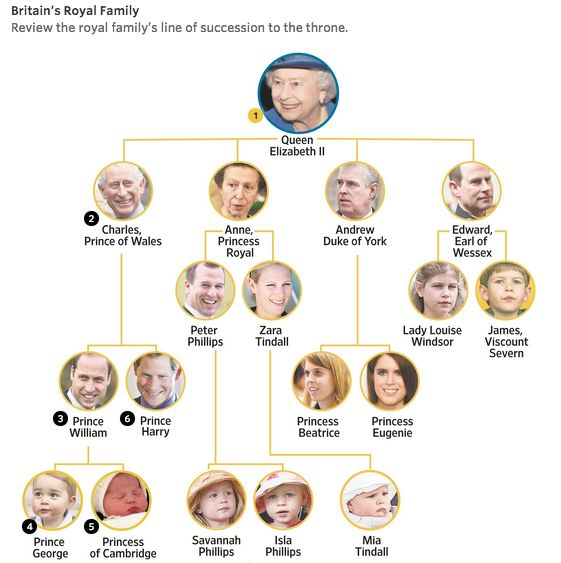
\includegraphics[width=0.6\textwidth]{fig/BritiansRoyalFamily.jpg}
        \caption{Britain's Royal Family}
        \label{fig:family}
    \end{figure}
    
    \part[1] \sone Using the tree shown in Figure \ref{fig:family}, how many nodes would depth-first-search visit in finding Mia Tindall (including her node)? Assume we search left-to-right and top-down.

    \begin{checkboxes}
        % YOUR ANSWER
        % Change \choice to \CorrectChoice for the appropriate selection/selections 
        \choice 3
        \CorrectChoice 12
        \choice 15
        \choice 18
    \end{checkboxes}

    
    \clearpage
    \part Figure \ref{tree} is a Binary Tree with indexed nodes. Assume root node is node 1. 
    
    \begin{figure}[H]
        \centering
        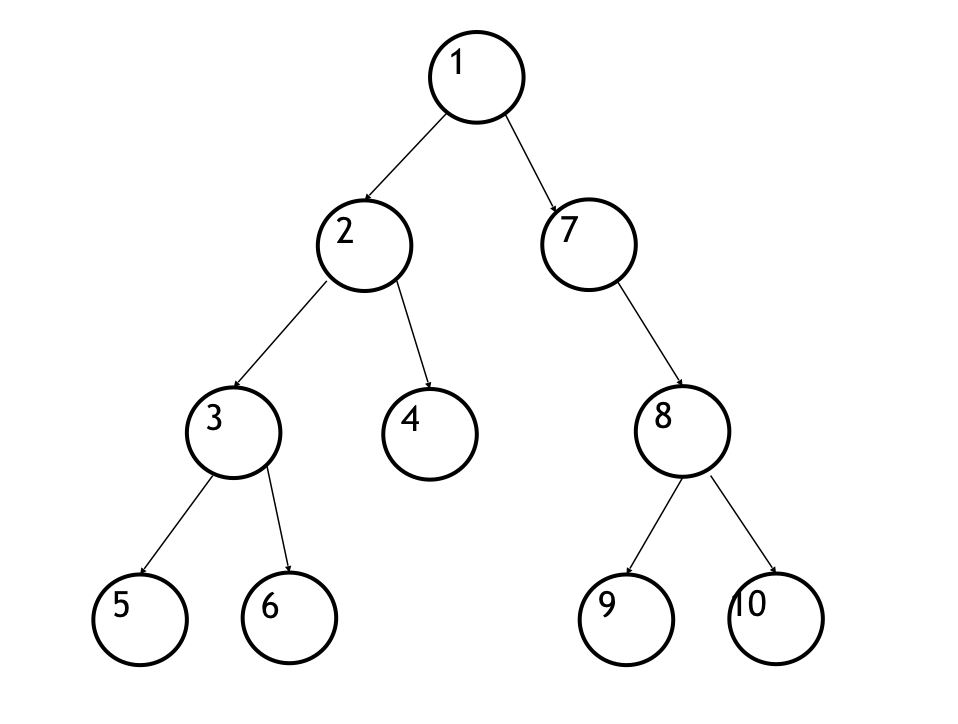
\includegraphics[width = 0.4\textwidth]{fig/TreePlot.png}
        \caption{A Binary Tree with indexed nodes}
        \label{tree}
    \end{figure}

    \begin{subparts}
    
    \subpart[1] What is the node-visit order of \textbf{DFS} and \textbf{BFS} of the above Binary Tree? 
    
    A depth-first search (DFS) traversal of a binary tree starts with visiting the root node, and recursively searches down the left subtree (i.e., the tree rooted at the left node) before going to search the right subtree (i.e., the tree rooted at the right node) until the traversal is done.\\
    Note: Alternatively, we can also look right subtree before left subtree too, for the question please consider left to right order!
    
    \begin{your_solution}[height=2cm, width=\textwidth, title={The node-visit order of DFS is (separate values with commas, e.g., 1,2,3,4)}]
    %solution
    1,2,3,5,6,4,7,8,9,10
    \end{your_solution}

    \subpart[1] What is the node-visit order of \textbf{BFS} of the above Binary Tree? 
    
    A breadth-first search (BFS) traversal of a binary tree visits every node (assuming a left-to-right order) on a level (with the same distance to the root) before going to a lower level until the traversal is done.
    
    \begin{your_solution}[height=2cm, width=\textwidth, title={The node-visit order of BFS is (separate values with commas, e.g., 1,2,3,4)}]
    %solution
    1,2,7,3,4,8,5,6,9,10
    \end{your_solution}
    
    \end{subparts}
    
    
    \clearpage
    
    \part[4] Fill in the blanks in the Python code for key search using recursive depth-first search (DFS) traversal. \emph{(Note: Please put your answer in the boxes below, not on the lines.)}
    
    \begin{lstlisting}[escapechar=@]
class TreeNode:
    def __init__(self, key):
        self.key = key
        self.leftNode = None
        self.rightNode = None
        
# (a) the left/right node is denoted as
#     node.leftNode/node.rightNode
# (b) left/right node are of type TreeNode
# (c) the key of the node is denoted as node.key
# (d) the left node is searched before the right node
        
def find_val(node, key):
    if node is None:
        return None
        
    if @\underline{~~\textbf{(1)}~~}@:
        return node
        
    else:
        result = @\underline{~~\textbf{(2)}~~}@
            
        if result is None:
            result = @\underline{~~\textbf{(3)}~~}@
            
        return @\underline{~~\textbf{(4)}~~}@
    \end{lstlisting}
    
    \begin{your_code_solution_outer}[height=1.75cm, width=\textwidth, title={Python code for missing field \textbf{(1)}}]
    % Put your solution in the your_code_solution environment
    \begin{your_code_solution}
    node.key == key
    \end{your_code_solution}
    \end{your_code_solution_outer}
    
    
    \begin{your_code_solution_outer}[height=1.75cm, width=\textwidth, title={Python code for missing field \textbf{(2)}}]
    % Put your solution in the your_code_solution environment
    \begin{your_code_solution}
    find_val(node.leftNode, key)
    \end{your_code_solution}
    \end{your_code_solution_outer}
    
    
    \begin{your_code_solution_outer}[height=1.75cm, width=\textwidth, title={Python code for missing field \textbf{(3)}}]
    % Put your solution in the your_code_solution environment
    \begin{your_code_solution}
    find_val(node.rightNode, key)
    \end{your_code_solution}
    \end{your_code_solution_outer}
    
    
    \begin{your_code_solution_outer}[height=1.75cm, width=\textwidth, title={Python code for missing field \textbf{(4)}}]
    % Put your solution in the your_code_solution environment
    \begin{your_code_solution}
    result
    \end{your_code_solution}
    \end{your_code_solution_outer}
    
    
\clearpage

\part Consider an $M \times N$ grid where each cell has a cost associated with passing through it. From any given cell, you can either travel to the right (same row, next column) or down (same column, next row). You need to return the minimum possible cost of traveling from the start point $[0, 0]$ in the top left of the grid to the end point $[M-1, N-1]$ in the bottom right of the grid. In Figure \ref{fig:example_grid}, the minimum cost path is highlighted in gold and the cost is $24$. Assume the cost of traveling outside the grid is infinite.

\begin{figure}[ht]
\centering
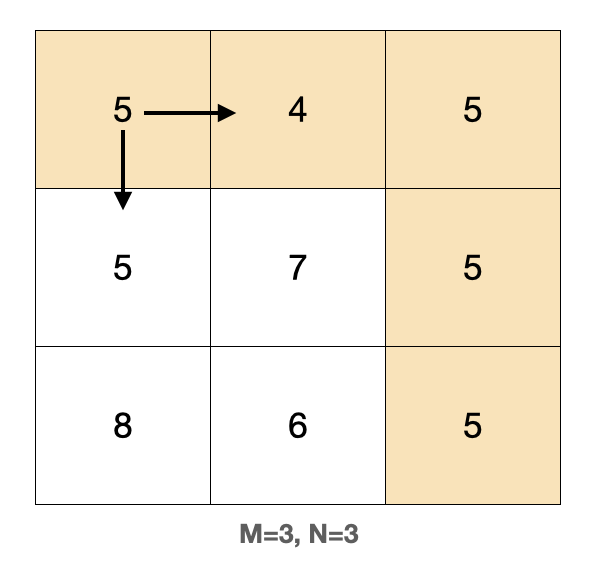
\includegraphics[scale=0.37]{fig/example_grid.png}
\caption{An example grid containing the costs for each cell and the directions one can travel from a cell.}
\label{fig:example_grid}
\end{figure}

We will first attempt to solve this using recursion. 

\begin{lstlisting}[escapechar=@]
# grid is of type List[List[int]]
m, n = len(grid), len(grid[0])


def minCostPath(r, c):
    if @\underline{~~\textbf{(1)}~~}@:
            return @\underline{~~\textbf{(2)}~~}@
                
    if r == m-1 and c == n-1:
        return grid[r][c]

    return @\underline{~~\textbf{(3)}~~}@

minCostPath(0, 0)
\end{lstlisting}
\begin{subparts}
\subpart[3] Fill in the blanks to complete the above function.

    \begin{your_code_solution_outer}[height=1.75cm, width=\textwidth, title={Python code for missing field \textbf{(1)}}]
    % Put your solution in the your_code_solution environment
    \begin{your_code_solution}
    r < 0 or r >= m or c < 0 or c >= n
    \end{your_code_solution}
    \end{your_code_solution_outer}

    \begin{your_code_solution_outer}[height=1.75cm, width=\textwidth, title={Python code for missing field \textbf{(2)}}]
    % Put your solution in the your_code_solution environment
    \begin{your_code_solution}
    float("inf")
    \end{your_code_solution}
    \end{your_code_solution_outer}

    \begin{your_code_solution_outer}[height=1.75cm, width=\textwidth, title={Python code for missing field \textbf{(3)}}]
    % Put your solution in the your_code_solution environment
    \begin{your_code_solution}
    grid[r][c] + min(minCostPath(r+1, c) + minCostPath(r, c+1))
    \end{your_code_solution}
    \end{your_code_solution_outer}



\subpart[3] From Figure \ref{fig:grid_memoize}, we can deduce that using recursion is inefficient because we recalculate the costs of different partial routes from the same intermediate cells to the endpoint.

The following figure demonstrates the inefficiency of using recursion to find the minimum cost path through the grid because it recalculates the cost of partial routes. For example, we can see that the red and black paths share the partial route from $[1,2]$ to $[2,2]$. The cost of this partial route is calculated once for the red path and once again for the black path.

\begin{figure}[ht]
\centering
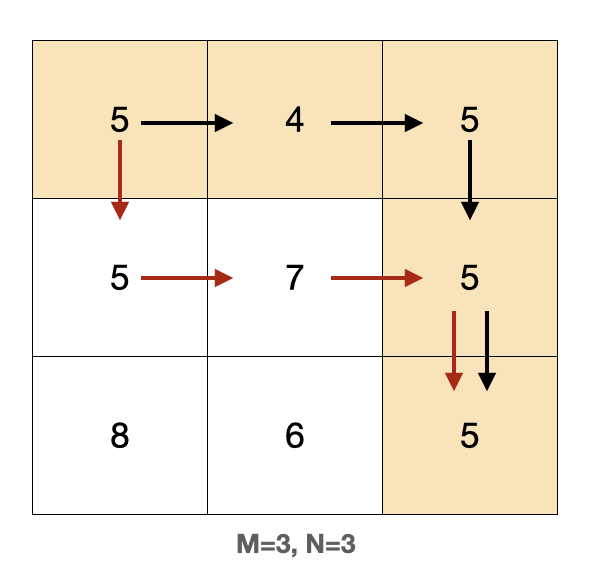
\includegraphics[scale=0.37]{fig/grid_memoize.png}
\caption{}
\label{fig:grid_memoize}
\end{figure}


To solve this problem, we can utilize memoization by creating a dictionary \texttt{cache} with each intermediate \texttt{r, c} state and its corresponding value of the \texttt{minCostPath} function.

Fill in the blanks below. \textbf{Assume fields (1) and (2) use your same solutions from above}.

\begin{lstlisting}[escapechar=@]
# grid is of type List[List[int]]
m, n = len(grid), len(grid[0])
cache = {}
        
def minCostPath(r, c):
        if @\underline{~~\textbf{(1)}~~}@:
            return @\underline{~~\textbf{(2)}~~}@

        if r == m-1 and c == n-1:
            return grid[r][c]

        key = (@\underline{~~\textbf{(4)}~~}@,@\underline{~~\textbf{(5)}~~}@)
        if key not in cache:
            cache[key] = @\underline{~~\textbf{(6)}~~}@
        return cache[key]

minCostPath(0, 0)
\end{lstlisting}
\vspace{-1em} % DO NOT REMOVE THIS LINE!

    \begin{your_code_solution_outer}[height=1.75cm, width=\textwidth/2, title=Your Python code for missing field \textbf{(4)}]
    % Put your solution in the your_code_solution environment
    \begin{your_code_solution}
    r
    \end{your_code_solution}
    \end{your_code_solution_outer}
   \begin{your_code_solution_outer}[height=1.75cm, width=\textwidth/2, title=Your Python code for missing field \textbf{(5)}]
    % Put your solution in the your_code_solution environment
    \begin{your_code_solution}
    c
    \end{your_code_solution}
    \end{your_code_solution_outer}

    \begin{your_code_solution_outer}[height=1.75cm, width=\textwidth, title=Your Python code for missing field \textbf{(6)}]
    % Put your solution in the your_code_solution environment
    \begin{your_code_solution}
    grid[r][c] + min(minCostPath(r+1, c), minCostPath(r, c+1))
    \end{your_code_solution}
    \end{your_code_solution_outer}
    

    
\end{subparts}

\end{parts}
\end{questions}
\newpage
\section{Collaboration Questions}
After you have completed all other components of this assignment, report your answers to these questions regarding the collaboration policy. Details of the policy can be found \href{http://www.cs.cmu.edu/~mgormley/courses/10601/syllabus.html}{here}.
\begin{enumerate}
    \item Did you receive any help whatsoever from anyone in solving this assignment? If so, include full details.
    \item Did you give any help whatsoever to anyone in solving this assignment? If so, include full details.
    \item Did you find or come across code that implements any part of this assignment ? If so, include full details.
\end{enumerate}

\begin{your_solution}[height=6cm]
% YOUR ANSWER 
\begin{enumerate}
    \item No.
    \item No.
    \item Yes, I find the following website (a) to clarify how to write 'infinite' number in Python, website (b) to figure out how to use min() built-in function, and website (c) to know how to use \textbackslash{url} to specify website in this answer block.
    \begin{enumerate}
    	\item \url{https://reurl.cc/0dZZKY}
	\item \url{https://www.w3schools.com/python/ref_func_min.asp}
	\item \url{https://stackoverflow.com/questions/2894710/how-to-write-urls-in-latex}
   \end{enumerate}
\end{enumerate}
\end{your_solution}


\end{document}